\documentclass[
  11pt,
  letterpaper,
   addpoints,
   answers
  ]{exam}

\usepackage[utf8]{inputenc}
\usepackage{../exercise-preamble}
\usepackage{float}
\usepackage{subcaption}
\usepackage{pgfplots}
\pgfplotsset{compat=1.18}
\usepgfplotslibrary{groupplots}
% TikZ libraries needed for `right=.. of ..` and coordinate math
\usetikzlibrary{positioning,calc,arrows,arrows.meta}

% Configuración de numeración de páginas
\makeatletter
\def\@oddfoot{\hfil Página \thepage \hfil}
\def\@evenfoot{\hfil Página \thepage \hfil}
\def\@oddhead{}
\def\@evenhead{}
\makeatother

\begin{document}

% Configuración del encabezado usando comandos de la clase exam
\pagestyle{headandfoot}
\extraheadheight{0.5in} % Baja el encabezado aumentando el espacio superior
\firstpageheader{\textit{Análisis de señales}}{}{EL3203}
\runningheader{\textit{Análisis de señales}}{}{EL3203}
\firstpagefooter{}{\thepage}{}
\runningfooter{}{\thepage}{}
\headrule % Línea debajo del encabezado

% Numeración de página
\pagenumbering{arabic}

% Portada
\begin{center}
    \vspace*{1cm}
    
    % Logo superior
    \includegraphics[width=0.5\textwidth]{../fcfm_die}
    
    \vspace{2cm}
    
    % Líneas decorativas superiores
    
\begin{tikzpicture}
        \draw[line width=2pt, black!70] (0,0) -- (10,0);
        \draw[line width=0.5pt, black!50] (0,0.2) -- (10,0.2);
    \end{tikzpicture}
    
    \vspace{1cm}
    
    % Título principal
    {\fontsize{28}{34}\selectfont\bfseries 
   Análisis de señales}
    
    \vspace{0.5cm}
    
    {\Large\textbf{EL3203}}
    
    \vspace{1cm}
    
    % Líneas decorativas inferiores
    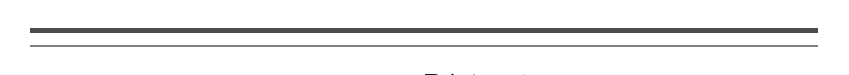
\begin{tikzpicture}
        \draw[line width=0.5pt, black!50] (0,0) -- (10,0);
        \draw[line width=2pt, black!70] (0,0.2) -- (10,0.2);
    \end{tikzpicture}
    
    \vspace{1.5cm}
    
    % Subtítulo
    {\LARGE\itshape Pauta Auxiliar 7 - Teorema del Muestreo}
    
    \vspace{0.5cm}
    {\large Prof Jorge Silva.}\\
    {\large Prof Auxiliar Erik Sáez Aravena.}
    
    \vfill
    

    \vspace{1cm}
    
\end{center}

\newpage
%----------------------------
\section{Resumen}

\subsection*{Transformadas de Fourier}

\textbf{Transformada de Fourier en tiempo discreto:}
\begin{equation}
  X(\omega) = \sum_{n \in \mathbb{Z}} x(n)e^{-j\omega n}
\end{equation}

\textbf{Transformada de Fourier en tiempo continuo:}
\begin{equation}
  X_a(\omega) = \int_{\mathbb{R}} x_a(t)e^{-j\omega t} d\omega
\end{equation}

\subsection*{Transformadas inversas de Fourier}

\textbf{Transformada inversa en tiempo discreto:}
\begin{equation}
  x(n) = \frac{1}{2\pi} \int_{-\pi}^{\pi} X(\omega)e^{j\omega n} d\omega
\end{equation}

\textbf{Transformada inversa en tiempo continuo:}
\begin{equation}
  x_a(t) = \frac{1}{2\pi} \int_{\mathbb{R}} X_a(\omega)e^{j\omega t} d\omega
\end{equation}

\subsection*{Espectro de señal muestreada}

El teorema del muestreo establece que cuando una señal analógica $x_a(t)$ se muestrea con periodo $T_s$ (frecuencia de muestreo $F_s = T_s^{-1}$), el espectro de frecuencia de la señal muestreada $X(2\pi f)$ está dado por:

\begin{equation}
  X(2\pi f) = F_s \sum_{k \in \mathbb{Z}} X_a(fF_s + kF_s)
\end{equation}

donde $f = \frac{F}{F_s}$ es la frecuencia normalizada.

\textbf{Cuando se muestrea por sobre la tasa de Nyquist}, no hay aliasing y tenemos:
\begin{equation}
  X(2\pi f) = F_s X_a(fF_s)
\end{equation}

Notemos que la señal $x(n)$ inducida por un muestreo con periodo $T_s$ está dada por:
\begin{equation}
  x(n) = x_a(nT_s)
\end{equation}

Además, sabemos que, por el teorema del muestreo, se cumple que el espectro de frecuencia de la señal muestreada $X(2\pi f)$ está dado por la suma infinita de réplicas desplazadas de $X_a$:
\begin{equation}
  X(2\pi f) = \sum_{k \in \mathbb{Z}} F_s X_a(fF_s + kF_s)
\end{equation}

donde $F_s = T_s^{-1}$ es la frecuencia de muestreo. Esta expresión viene de considerar que, dado que la señal es discreta, la TF de la señal discreta es periódica con periodo 1, por lo que la TF en una frecuencia particular se ve afectada por las infinitas bandas laterales.

\subsection*{Condición de Nyquist}

Para poder recuperar perfectamente la señal analógica original $x_a(t)$ a partir de sus muestras $x(n)$, debe cumplirse:
\begin{equation}
  F_s \geq 2B
\end{equation}

donde $B$ es el ancho de banda de la señal (frecuencia máxima presente en la señal). Si esta condición no se cumple, ocurre \textbf{aliasing} y la señal no puede recuperarse.

\subsection*{Función sinc}

La función sinc normalizada se define como:
\begin{equation}
  \text{sinc}(\pi x) = \frac{\sin(\pi x)}{\pi x}
\end{equation}

Esta función aparece naturalmente en problemas de muestreo e interpolación.

\newpage

\begin{questions}

\question Sea $x_a(t)$ una señal analógica de banda limitada con transformada de Fourier $X_a(F)$ y período de muestreo $T_s = \frac{1}{F_s}$. Se define la señal discreta muestreada como $x(n) = x_a(nT_s)$ para $n \in \mathbb{Z}$.

\begin{parts}
  \part Demuestre que la transformada de Fourier discreta $X(\omega)$ de la señal muestreada puede escribirse en términos de la transformada continua como:
  \begin{equation}
    X(\omega) = \sum_{n=-\infty}^{\infty} x_a(nT_s)e^{-j\omega n}
  \end{equation}
  
  y que esta se relaciona con $X_a(F)$ mediante:
  \begin{equation}
    X(2\pi f) = F_s \sum_{k=-\infty}^{\infty} X_a(fF_s + kF_s)
  \end{equation}
  
  donde $f = \frac{F}{F_s}$ es la frecuencia normalizada.
  
  \begin{solution}
  
    Sabemos que la transformada inversa de Fourier continua está dada por:
    \begin{equation}
      x_a(t) = \int_{-\infty}^{\infty} X_a(F)e^{\left(j2\pi Ft\right)} dF
    \end{equation}
    
    Evaluando en $t = nT_s$ y usando $F_s = T_s^{-1}$:
    \begin{equation}
      x(n) = x_a(nT_s) = \int_{-\infty}^{\infty} X_a(F)e^{\left(j2\pi \frac{F}{F_s}n\right)} dF
    \end{equation}
    
    Por otro lado, la transformada inversa de Fourier discreta está dada por:
    \begin{equation}
      x(n) = \int_{-\frac{1}{2}}^{\frac{1}{2}} X(2\pi f)e^{\left(j2\pi fn\right)} df
    \end{equation}
    
    Por lo tanto, tenemos la siguiente identidad:
    \begin{equation}
      \int_{-\frac{1}{2}}^{\frac{1}{2}} X(2\pi f) e^{\left(j2\pi fn\right)} df = \int_{-\infty}^{\infty} X_a(F)e^{\left(j2\pi \frac{F}{F_s}n\right)} dF
    \end{equation}
    
    Definimos la siguiente función indexada por $F$:
    \begin{equation}
      \Phi_F(n) = e^{\left(j2\pi \frac{F}{F_s}n\right)}
    \end{equation}
    
    Esta función tiene las siguientes propiedades de periodicidad:
    \begin{align}
      \Phi_{F+F_s}(n) &= e^{\left(j2\pi \frac{F+F_s}{F_s}n\right)} = e^{\left(j2\pi \frac{F}{F_s}n\right)} \cdot e^{\left(j2\pi n\right)} = \Phi_F(n) \quad \forall n \in \mathbb{Z}\\
      \Phi_{F+\ell F_s}(n) &= \Phi_F(n) \quad \forall n \in \mathbb{Z}, \forall \ell \in \mathbb{Z}
    \end{align}
    
    Por lo tanto, podemos descomponer la integral sobre toda la recta real como suma de integrales sobre intervalos de longitud $F_s$:
    \begin{equation}
      \int_{-\infty}^{\infty} X_a(F)\Phi_F(n) dF = \sum_{k \in \mathbb{Z}} \int_{-\frac{F_s}{2} + kF_s}^{\frac{F_s}{2} + kF_s} X_a(F)\Phi_F(n) dF
    \end{equation}
    
    Realizando el cambio de variable $\hat{F} = F - kF_s$ (entonces $dF = d\hat{F}$), tenemos:
    \begin{align}
      \int_{-\infty}^{\infty} X_a(F)\Phi_F(n) dF &= \sum_{k \in \mathbb{Z}} \int_{-\frac{F_s}{2}}^{\frac{F_s}{2}} X_a(\hat{F} + kF_s) \cdot \Phi_{\hat{F}+kF_s}(n) d\hat{F}\\
      &= \sum_{k \in \mathbb{Z}} \int_{-\frac{F_s}{2}}^{\frac{F_s}{2}} X_a(\hat{F} + kF_s) \cdot \Phi_{\hat{F}}(n) d\hat{F}\\
      &= \int_{-\frac{F_s}{2}}^{\frac{F_s}{2}} \left[\sum_{k \in \mathbb{Z}} X_a(\hat{F} + kF_s)\right] \cdot \Phi_{\hat{F}}(n) d\hat{F}\\
      &= \int_{-\frac{F_s}{2}}^{\frac{F_s}{2}} \left[\sum_{k \in \mathbb{Z}} X_a(\hat{F} + kF_s)\right] \cdot e^{\left(j2\pi \frac{\hat{F}}{F_s}n\right)} d\hat{F}
    \end{align}
    
    donde en el segundo paso usamos la propiedad de periodicidad $\Phi_{\hat{F}+kF_s}(n) = \Phi_{\hat{F}}(n)$. Ahora realizamos el cambio de variable $f = \frac{\hat{F}}{F_s}$ (frecuencia normalizada), por lo que $d\hat{F} = F_s df$:
    \begin{align}
      \int_{-\infty}^{\infty} X_a(F)\Phi_F(n) dF &= \int_{-\frac{1}{2}}^{\frac{1}{2}} \left[\sum_{k \in \mathbb{Z}} X_a(fF_s + kF_s)\right] \cdot e^{\left(j2\pi fn\right)} \cdot F_s df\\
      &= \int_{-\frac{1}{2}}^{\frac{1}{2}} F_s \left[\sum_{k \in \mathbb{Z}} X_a(fF_s + kF_s)\right] e^{\left(j2\pi fn\right)} df
    \end{align}
    
    Comparando con la identidad que establecimos anteriormente:
    \begin{equation}
      \int_{-\frac{1}{2}}^{\frac{1}{2}} X(2\pi f) e^{\left(j2\pi fn\right)} df = \int_{-\frac{1}{2}}^{\frac{1}{2}} F_s \left[\sum_{k \in \mathbb{Z}} X_a(fF_s + kF_s)\right] e^{\left(j2\pi fn\right)} df
    \end{equation}
    
    Como esta igualdad debe cumplirse para todo $n \in \mathbb{Z}$, y dado que $e^{\left(j2\pi fn\right)}$ forma una base ortogonal, concluimos que:
    \begin{equation}
      \boxed{X(2\pi f) = F_s \sum_{k=-\infty}^{\infty} X_a(fF_s + kF_s)}
    \end{equation}
    
    para $f \in (-1/2, 1/2]$. Esta es la relación fundamental entre el espectro de la señal muestreada y el espectro de la señal continua original.
   
  \end{solution}
  
  \part Para la señal anterior, demuestre que bajo la condición de muestreo de Nyquist ($F_s \geq 2B$, donde $B$ es el ancho de banda de la señal), la relación se simplifica a:
  \begin{equation}
    X(2\pi f) = F_s X_a(fF_s), \quad \text{para } f \in (-1/2, 1/2]
  \end{equation}
  
  y que por lo tanto es posible recuperar la señal original mediante:
  \begin{equation}
    x_a(t) = T_s \sum_{k \in \mathbb{Z}} x_a(kT_s) \text{sinc}\left(\pi\frac{t - kT_s}{T_s}\right)
  \end{equation}
  
  \begin{solution}
    Del resultado de la parte (a), tenemos:
    \begin{equation}
      X(2\pi f) = F_s\sum_{k=-\infty}^{\infty} X_a(fF_s + kF_s)
    \end{equation}
    
    Si la señal $x_a(t)$ es de banda limitada con ancho de banda $B$, entonces:
    \begin{equation}
      X_a(F) = 0 \quad \text{para } |F| > B
    \end{equation}
    
    Cuando se cumple la condición de Nyquist $F_s \geq 2B$, analicemos cuándo los términos $X_a(fF_s + kF_s)$ son no nulos en el intervalo fundamental $f \in (-1/2, 1/2]$.
    
    Para la banda $k$-ésima, necesitamos que:
    \begin{equation}
      |fF_s + kF_s| \leq B
    \end{equation}
    
    Para $f \in (-1/2, 1/2]$:
    \begin{equation}
      -\frac{F_s}{2} < fF_s \leq \frac{F_s}{2}
    \end{equation}
    
    Por lo tanto:
    \begin{equation}
      -\frac{F_s}{2} + kF_s < fF_s + kF_s \leq \frac{F_s}{2} + kF_s
    \end{equation}
    
    Para que $|fF_s + kF_s| \leq B$, necesitamos que los intervalos $\left(-\frac{F_s}{2} + kF_s, \frac{F_s}{2} + kF_s\right]$ se intersecten con $[-B, B]$.
    
    Para $k = 0$: El intervalo es $(-F_s/2, F_s/2]$. Dado que $F_s \geq 2B$, tenemos $[-B, B] \subseteq (-F_s/2, F_s/2]$, por lo que este término contribuye.
    
    Para $k \neq 0$: Los intervalos están centrados en $kF_s$ con ancho $F_s$. Para $k = 1$, el límite inferior es $F_s/2$ y para $k = -1$, el límite superior es $-F_s/2$. Dado que $F_s \geq 2B$, tenemos:
    \begin{equation}
      \frac{F_s}{2} \geq B \quad \text{y} \quad -\frac{F_s}{2} \leq -B
    \end{equation}
    
    Por lo tanto, no hay intersección entre las bandas adyacentes y $[-B, B]$ en el intervalo fundamental. Así:
    \begin{equation}
      \boxed{X(2\pi f) = F_s X_a(fF_s), \quad f \in (-1/2, 1/2]}
    \end{equation}
    
    
    Para recuperar $x_a(t)$, partimos de la transformada inversa de Fourier continua:
    \begin{equation}
      x_a(t) = \int_{-\infty}^{\infty} X_a(F)e^{\left(j2\pi Ft\right)} dF
    \end{equation}
    
    Dado que $X_a(F) = 0$ para $|F| > B$ y $B \leq F_s/2$ (condición de Nyquist), podemos limitar la integración:
    \begin{equation}
      x_a(t) = \int_{-\frac{F_s}{2}}^{\frac{F_s}{2}} X_a(F)e^{\left(j2\pi Ft\right)} dF
    \end{equation}
    
    Haciendo el cambio de variable $f = \frac{F}{F_s}$ (entonces $dF = F_s df$):
    \begin{equation}
      x_a(t) = \int_{-\frac{1}{2}}^{\frac{1}{2}} X_a(fF_s)e^{\left(j2\pi fF_s t\right)} F_s df
    \end{equation}
    
    Usando la relación simplificada $X_a(fF_s) = \frac{1}{F_s}X(2\pi f)$ obtenida bajo la condición de Nyquist:
    \begin{equation}
      x_a(t) = \int_{-\frac{1}{2}}^{\frac{1}{2}} \frac{1}{F_s}X(2\pi f)e^{\left(j2\pi fF_s t\right)} F_s df = \int_{-\frac{1}{2}}^{\frac{1}{2}} X(2\pi f)e^{\left(j2\pi fF_s t\right)} df
    \end{equation}
    
    De la parte (a), sabemos que la transformada de Fourier discreta está dada por:
    \begin{equation}
      X(2\pi f) = \sum_{n=-\infty}^{\infty} x(n)e^{\left(-j2\pi fn\right)} = \sum_{n=-\infty}^{\infty} x_a(nT_s)e^{\left(-j2\pi fn\right)}
    \end{equation}
    
    Sustituyendo esta expresión en la integral:
    \begin{align}
      x_a(t) &= \int_{-\frac{1}{2}}^{\frac{1}{2}} \left[\sum_{n=-\infty}^{\infty} x_a(nT_s)e^{\left(-j2\pi fn\right)}\right] e^{\left(j2\pi fF_s t\right)} df \\
      &= \sum_{n=-\infty}^{\infty} x_a(nT_s) \int_{-\frac{1}{2}}^{\frac{1}{2}} e^{\left(j2\pi f(F_s t - n)\right)} df
    \end{align}
    
    donde hemos intercambiado la suma y la integral (por convergencia uniforme).
    
    Calculando la integral:
    \begin{align}
      \int_{-\frac{1}{2}}^{\frac{1}{2}} e^{\left(j2\pi f(F_s t - n)\right)} df &= \frac{1}{j2\pi(F_s t - n)}\left[e^{\left(j\pi(F_s t - n)\right)} - e^{\left(-j\pi(F_s t - n)\right)}\right] \\
      &= \frac{1}{j2\pi(F_s t - n)} \cdot j2\sin(\pi(F_s t - n)) \\
      &= \frac{\sin(\pi(F_s t - n))}{\pi(F_s t - n)} \\
      &= \text{sinc}(\pi(F_s t - n))
    \end{align}
    
    Por lo tanto, sustituyendo en la expresión de $x_a(t)$:
    \begin{equation}
      x_a(t) = \sum_{n=-\infty}^{\infty} x_a(nT_s) \text{sinc}(\pi(F_s t - n))
    \end{equation}
    
    Usando $F_s = T_s^{-1}$, podemos reescribir $F_s t - n = \frac{t - nT_s}{T_s}$, por lo que:
    \begin{equation}
      x_a(t) = \sum_{n=-\infty}^{\infty} x_a(nT_s) \text{sinc}\left(\pi\frac{t - nT_s}{T_s}\right)
    \end{equation}
    
    Haciendo el cambio de índice $k = n$, obtenemos finalmente:
    \begin{equation}
      \boxed{x_a(t) = \sum_{k=-\infty}^{\infty} x_a(kT_s) \text{sinc}\left(\pi\frac{t - kT_s}{T_s}\right)}
    \end{equation}
    
    que también puede escribirse multiplicando y dividiendo por $T_s$:
    \begin{equation}
      x_a(t) = T_s \sum_{k=-\infty}^{\infty} x_a(kT_s) \text{sinc}\left(\pi\frac{t - kT_s}{T_s}\right)
    \end{equation}
    
    Esta es la fórmula de Shannon, que demuestra que bajo la condición de Nyquist, la señal analógica original puede reconstruirse perfectamente como una suma infinita de funciones sinc centradas en los instantes de muestreo, ponderadas por los valores de las muestras.
  \end{solution}
\end{parts}
%------------------------
  \question Considere una señal $x_a(t)$ con transformada de Fourier como se muestra en la figura
  
  \begin{figure}[H]
    \centering
    \begin{tikzpicture}
      \begin{axis}[
        axis lines=middle,
        xlabel={$F$},
        ylabel={$X_a(F)$},
        xmin=-2.5, xmax=2.5,
        ymin=-0.2, ymax=1.5,
        xtick={-2,-1,0,1,2},
        xticklabels={$-2F_0$,$-F_0$,$0$,$F_0$,$2F_0$},
        ytick={1},
        width=10cm,
        height=6cm,
      ]
      % Rectángulo izquierdo
      \addplot[thick, fill=black!20, pattern=north east lines] coordinates {
        (-2,0) (-2,1) (-1,1) (-1,0) (-2,0)
      };
      % Rectángulo derecho
      \addplot[thick, fill=black!20, pattern=north east lines] coordinates {
        (1,0) (1,1) (2,1) (2,0) (1,0)
      };
      \end{axis}
    \end{tikzpicture}
    \caption{Transformada de Fourier de la señal $x_a(t)$.}
  \end{figure}
  
  \begin{parts}
    \part Considere un proceso de muestreo donde $F_s = 4F_0$. Encuentre una expresión para $x(n)$. \textbf{Indicación:} Utilice la relación entre $X_a(F)$ y $X(2\pi f) = \text{DTFT}\{x(n)\}$ dadas por el teorema del muestreo.
    
    \begin{solution}
    
      Notemos que la señal $x(n)$ inducida por un muestreo con período $T_s$ está dada por:
      \begin{equation}
        x(n) = x_a(nT_s), \quad n \in \mathbb{Z}
      \end{equation}
      
      Además, sabemos que, por el teorema del muestreo (demostrado en la parte (a)), se cumple que el espectro de frecuencia de la señal muestreada $X(2\pi f)$ está dado por:
      \begin{equation}
        X(2\pi f) = \sum_{k \in \mathbb{Z}} F_s X_a(fF_s + kF_s),
      \end{equation}
      
      donde $F_s = T_s^{-1}$ es la frecuencia de muestreo. Esta expresión viene de considerar que, dado que la señal es discreta, la TF de la señal discreta es periódica con periodo 1, por lo que la TF en una frecuencia particular se ve afectada por las infinitas bandas laterales.
      
      Notemos que, para la señal analógica original, a partir de la TF visual se puede ver que:
      \begin{equation}
        \text{supp}(X_a(f)) = [-2F_0, -F_0] \cup [F_0, 2F_0]
      \end{equation}
      Donde $\text{supp}(\cdot)$ denota el soporte de la función, es decir el conjunto donde la función es no nula.
  
      
      Para la $k$-ésima banda, la TF discreta está dada por $X_a(fF_s + kF_s)$, por lo que podemos calcular el soporte de cada banda y analizar cuáles de ellas tienen intersección con el intervalo fundamental $(-1/2, 1/2]$, de modo que aquellas bandas cuya intersección es nula pueden ser omitidas de la sumatoria. 
      
      Para calcular el soporte, debemos obtener los valores de frecuencia $f_k^{\text{low}}$ y $f_k^{\text{high}}$ que entregan los límites inferiores y superiores, respectivamente, del soporte de la señal analógica. Haciendo esto, notemos que estos deben ser tales que:
      \begin{equation}
        f_k^{\text{low}}F_s + kF_s = -2F_0 \quad \land \quad f_k^{\text{high}}F_s + kF_s = 2F_0
      \end{equation}
      
      Calculando cada uno, considerando que $F_s = 4F_0$, tenemos:
      \begin{align}
        f_k^{\text{low}}F_s + kF_s &= -2F_0 \\
        \Leftrightarrow 4f_k^{\text{low}}F_0 + 4kF_0 &= -2F_0 \\
        \Leftrightarrow 4f_k^{\text{low}} + 4k &= -2 \\
        \Leftrightarrow f_k^{\text{low}} &= -\frac{1}{2} - k
      \end{align}
      
      Para la frecuencia superior, haciendo un análisis similar se puede ver que $f_k^{\text{high}} = \frac{1}{2} - k$, por lo que:
      \begin{equation}
        \text{supp}(X_a(fF_s + kF_s)) = \left(-\frac{1}{2} - k, \frac{1}{2} - k\right]
      \end{equation}
      
      de lo que podemos ver que el único valor de $k$ para el cual el soporte tiene intersección no nula con el intervalo fundamental es $k = 0$. De este modo, la TF de la señal muestreada se simplifica a:
      \begin{equation}
        X(2\pi f) = F_s X_a(fF_s) = 4F_0 X_a(4fF_0)
      \end{equation}
      
      \begin{figure}[H]
        \centering
        \begin{tikzpicture}
          \begin{axis}[
            axis lines=middle,
            xlabel={$f$},
            ylabel={$X(2\pi f)$},
            xmin=-0.6, xmax=0.6,
            ymin=-0.2, ymax=5,
            xtick={-0.5,-0.25,0,0.25,0.5},
            xticklabels={$-\frac{1}{2}$,$-\frac{1}{4}$,$0$,$\frac{1}{4}$,$\frac{1}{2}$},
            ytick={4},
            yticklabels={$4F_0$},
            width=12cm,
            height=6cm,
          ]
          % Rectángulo izquierdo
          \addplot[thick, fill=blue!20, pattern=north east lines, pattern color=blue] coordinates {
            (-0.5,0) (-0.5,4) (-0.25,4) (-0.25,0) (-0.5,0)
          };
          % Rectángulo derecho
          \addplot[thick, fill=blue!20, pattern=north east lines, pattern color=blue] coordinates {
            (0.25,0) (0.25,4) (0.5,4) (0.5,0) (0.25,0)
          };
          \end{axis}
        \end{tikzpicture}
        \caption{Espectro de la señal muestreada $X(2\pi f)$ para $F_s = 4F_0$ (sin aliasing).}
      \end{figure}
      
      la cual, en base a la representación gráfica de $X_a(f)$, podemos escribir como:
      \begin{equation}
        X(2\pi f) = \begin{cases}
          4F_0 & \text{si } f \in (-1/2, -1/4] \\
          0 & \text{si } f \in (-1/4, 1/4] \\
          4F_0 & \text{si } f \in (1/4, 1/2]
        \end{cases}
      \end{equation}
  
      Luego, podemos aplicar la inversa de Fourier para obtener la señal en el dominio del tiempo, de lo que tenemos:
      \begin{align}
        x(n) &= \int_{-1/2}^{1/2} X(2\pi f)e^{\left(j2\pi fn\right)} df \\
        &= 4F_0 \int_{-1/2}^{-1/4} e^{\left(j2\pi fn\right)} df + 4F_0 \int_{1/4}^{1/2} e^{\left(j2\pi fn\right)} df \\
        &= \frac{4F_0}{j2\pi n} \left[e^{\left(-j\frac{\pi}{2}n\right)} - e^{\left(-j\pi n\right)} + e^{\left(j\pi n\right)} - e^{\left(j\frac{\pi}{2}n\right)}\right]
      \end{align}
      
      Notemos que las exponenciales se pueden agrupar, considerando que:
      \begin{equation}
        \sin(\theta) = \frac{e^{\left(j\theta\right)} - e^{\left(-j\theta\right)}}{j2}
      \end{equation}
      
      por lo que tenemos:
      \begin{equation}
        x(n) = \frac{4F_0}{j2\pi n} \left[j2\sin(\pi n) - j2\sin\left(\frac{\pi}{2}n\right)\right] = \frac{4F_0}{\pi n} \left[\sin(\pi n) - \sin\left(\frac{\pi}{2}n\right)\right]
      \end{equation}
      
      Luego, notemos que, dado que $n \in \mathbb{Z}$, se tiene $\sin(\pi n) = 0$, por lo que ese término no se considera dentro de la expresión. Así, finalmente tenemos que la señal muestreada está dada por:
      \begin{equation}
        \boxed{x(n) = -4F_0 \frac{\sin\left(\frac{\pi}{2}n\right)}{\pi n}}
      \end{equation}
      
      Notemos además que, considerando la función sinc la cual está definida como:
      \begin{equation}
        \text{sinc}(\pi x) = \frac{\sin(\pi x)}{\pi x}
      \end{equation}
      
      podemos escribir la señal en términos de esta función como:
      \begin{equation}
        x(n) = -2F_0 \text{sinc}\left(\frac{\pi}{2}n\right)
      \end{equation}
    \end{solution}
    
    \part Repita el análisis del punto anterior si $F_s = 3F_0$ y comente si es posible recuperar $x_a(t)$ a partir de $x(n)$
    
    \begin{solution}
      \textbf{Muestreo con $F_s = 3F_0$}
      
      El procedimiento a seguir para este caso es análogo al usado para la frecuencia anterior. En este caso, notemos que para la $k$-ésima banda las frecuencias máximas y mínimas son:
      \begin{align}
        3f_k^{\text{low}}F_0 + 3kF_0 &= -2F_0 \\
        \Leftrightarrow 3f_k^{\text{low}} + 3k &= -2 \\
        \Leftrightarrow f_k^{\text{low}} &= -\frac{2}{3} - k
      \end{align}
      
      \begin{align}
        3f_k^{\text{high}}F_0 + 3kF_0 &= 2F_0 \\
        \Leftrightarrow 3f_k^{\text{high}} + 3k &= 2 \\
        \Leftrightarrow f_k^{\text{high}} &= \frac{2}{3} - k
      \end{align}
      
      por lo que el soporte de la $k$-ésima banda es:
      \begin{equation}
        \text{supp}(X_a(3fF_0 + 3kF_0)) = \left(-\frac{2}{3} - k, \frac{2}{3} - k\right]
      \end{equation}
      
      En este caso, a diferencia del caso anterior, notemos que las bandas $k = 1$ y $k = -1$ \textbf{sí intersectan} al intervalo fundamental, ya que los soportes de estas dos bandas son $(-5/3, -1/3]$ y $(1/3, 5/3]$, respectivamente. Esto significa que, ahora, al reconstruir el espectro discreto debemos considerar estos dos términos en la sumatoria, por lo que tenemos:
      \begin{equation}
        X(2\pi f) = 3F_0 [X_a(3fF_0 - 3F_0) + X_a(3fF_0) + X_a(3fF_0 + 3F_0)]
      \end{equation}
      
      \begin{figure}[H]
        \centering
        \begin{tikzpicture}
          \begin{axis}[
            axis lines=middle,
            xlabel={$f$ },
            ylabel={$X(2\pi f)$},
            xmin=-0.6, xmax=0.6,
            ymin=-0.2, ymax=7,
            xtick={-0.5,-0.333,0,0.333,0.5},
            xticklabels={$-\frac{1}{2}$,$-\frac{1}{3}$,$0$,$\frac{1}{3}$,$\frac{1}{2}$},
            ytick={3,6},
            yticklabels={$3F_0$,$6F_0$},
            width=12cm,
            height=6cm,
          ]
          % Banda k=-1 (roja, parcialmente fuera)
          \addplot[thick, fill=red!20, pattern=dots, pattern color=red, opacity=0.7] coordinates {
            (-0.6,0) (-0.6,3) (-0.333,3) (-0.333,0) (-0.6,0)
          };
          \node[red] at (axis cs:-0.47,3.5) {\small $k=-1$};
          
          % Banda k=0 (azul, central)
          \addplot[thick, fill=blue!20, pattern=north east lines, pattern color=blue, opacity=0.7] coordinates {
            (-0.5,0) (-0.5,3) (-0.333,3) (-0.333,0) (-0.5,0)
          };
          \addplot[thick, fill=blue!20, pattern=north east lines, pattern color=blue, opacity=0.7] coordinates {
            (0.333,0) (0.333,3) (0.5,3) (0.5,0) (0.333,0)
          };
          \node[blue] at (axis cs:0,3.5) {\small $k=0$};
          
          % Banda k=1 (verde, parcialmente fuera)
          \addplot[thick, fill=green!30, pattern=dots, pattern color=green!70!black, opacity=0.7] coordinates {
            (0.333,0) (0.333,3) (0.6,3) (0.6,0) (0.333,0)
          };
          \node[green!70!black] at (axis cs:0.47,3.5) {\small $k=1$};
          
          % Superposición (aliasing) - regiones con doble altura
          \addplot[thick, fill=orange!40, pattern=crosshatch, pattern color=orange!70!red] coordinates {
            (-0.5,3) (-0.5,6) (-0.333,6) (-0.333,3) (-0.5,3)
          };
          \addplot[thick, fill=orange!40, pattern=crosshatch, pattern color=orange!70!red] coordinates {
            (0.333,3) (0.333,6) (0.5,6) (0.5,3) (0.333,3)
          };
          
          % Marcadores de aliasing
          \node[orange!70!red, font=\scriptsize] at (axis cs:-0.417,5) {Aliasing};
          \node[orange!70!red, font=\scriptsize] at (axis cs:0.417,5) {Aliasing};
          
          \end{axis}
        \end{tikzpicture}
        \caption{Espectro de la señal muestreada $X(2\pi f)$ para $F_s = 3F_0$ mostrando el aliasing. Las regiones naranjas indican la superposición de bandas.}
      \end{figure}
      
      Al escribir este espectro considerando la representación gráfica de $X_a(f)$, tenemos:
      \begin{equation}
        X(2\pi f) = \begin{cases}
          6F_0 & \text{si } f \in \left(-\frac{1}{2}, -\frac{1}{3}\right] \\[0.3cm]
          0 & \text{si } f \in \left(-\frac{1}{3}, \frac{1}{3}\right] \\[0.3cm]
          6F_0 & \text{si } f \in \left(\frac{1}{3}, \frac{1}{2}\right]
        \end{cases}
      \end{equation}
      
      donde notemos que se tiene $6F_0$ en vez de $3F_0$ ya que, a diferencia de la señal anterior, en este caso las componentes de las bandas adyacentes se superponen, haciendo que tengan una mayor amplitud.
      
      
      Luego, podemos aplicar la inversa de Fourier al igual que hicimos con la señal anterior, de donde tenemos:
      \begin{align}
        x(n) &= \int_{-1/2}^{1/2} X(2\pi f)e^{\left(j2\pi fn\right)} df \\
        &= 6F_0 \left[\int_{-1/2}^{-1/3} e^{\left(j2\pi fn\right)} df + \int_{1/3}^{1/2} e^{\left(j2\pi fn\right)} df\right] \\
        &= \frac{6F_0}{j2\pi n} \left[e^{\left(-j\frac{2\pi}{3}n\right)} - e^{\left(-j\pi n\right)} + e^{\left(j\pi n\right)} - e^{\left(j\frac{2\pi}{3}n\right)}\right]
      \end{align}
      
      Al igual que antes, podemos agrupar términos para formar sinusoidales, de donde tenemos:
      \begin{align}
        x(n) &= \frac{6F_0}{j2\pi n} \left[j2\sin(\pi n) - j2\sin\left(\frac{2\pi}{3}n\right)\right] \\
        &= -6F_0 \frac{\sin\left(\frac{2\pi}{3}n\right)}{\pi n},
      \end{align}
      
      donde, al igual que en la señal anterior, se tiene $\sin(\pi n) = 0$. Por lo tanto:
      \begin{equation}
        \boxed{x(n) = -6F_0 \frac{\sin\left(\frac{2\pi}{3}n\right)}{\pi n}}
      \end{equation}
      
      Además, análogo al caso anterior, esta señal puede ser escrita usando la función sinc como:
      \begin{equation}
        x(n) = -4F_0 \text{sinc}\left(\frac{2\pi}{3}n\right)
      \end{equation}
      
      
      \textit{No es posible recuperar $x_a(t)$ a partir de $x(n)$ cuando $F_s = 3F_0$}, ya que hay \textbf{aliasing}. Las componentes de las bandas $k=1$ y $k=-1$ se superponen con la banda fundamental en los intervalos $(-1/2, -1/3]$ y $(1/3, 1/2]$ respectivamente, violando el teorema del muestreo que requiere:
      \begin{equation}
        F_s \geq 2B
      \end{equation}
      
      donde $B = 2F_0$ es el ancho de banda máximo de la señal (frecuencia máxima presente). En este caso:
      \begin{equation}
        F_s = 3F_0 < 4F_0 = 2B
      \end{equation}
      
      Por lo tanto, la condición de Nyquist \textbf{no se cumple} y la información original se pierde debido a la superposición espectral (aliasing).
    \end{solution}
  \end{parts}
  
  \question \textit{Muestreo natural.} Suponga que la señal $f(t)$ es de banda limitada con $\mathcal{F}f(s) = 0$ para $|s| \geq B$. En lugar de muestrear con un tren de $\delta$'s, muestreamos $f(t)$ con un tren de pulsos muy angostos. El pulso está dado por una función $p(t)$, muestreamos a una tasa $T$, y la señal muestreada tiene la forma
  \begin{equation}
    g(t) = f(t) \left( \sum_{k=-\infty}^{\infty} T p(t - kT) \right)
  \end{equation}
  
  \begin{parts}
    \part ¿Es posible recuperar la señal original $f$ a partir de la señal $g$?
    
    \part Si no es posible, ¿por qué no? Si es posible, ¿qué condiciones sobre los parámetros $T$ y $B$, y sobre el pulso $p(x)$ lo hacen posible?
    
    \begin{solution}
      Generalmente es más fácil pensar en el muestreo en el dominio de la frecuencia, por lo que comenzaremos encontrando la transformada de Fourier de $g(t)$. Notemos que nuestra función de muestreo natural es una periodización del pulso y puede expresarse como una convolución del pulso con un tren de impulsos.
      
      Podemos reescribir la señal muestreada como:
      \begin{align}
        g(t) &= f(t)T \sum_{n=-\infty}^{\infty} p(t - nT) \\
        &= f(t)T \left( p(t) \ast \sum_{n=-\infty}^{\infty} \delta(t - nT) \right)
      \end{align}
      
      donde en la segunda línea usamos la propiedad de que $\sum_{n=-\infty}^{\infty} p(t - nT) = p(t) \ast \sum_{n=-\infty}^{\infty} \delta(t - nT)$.
      
      Ahora, aplicamos la transformada de Fourier. Usando el teorema de convolución $\mathcal{F}\{f(t)h(t)\} = \mathcal{F}f(s) \ast \mathcal{F}h(s)$ y la propiedad dual del teorema de convolución, tenemos:
      \begin{align}
        \mathcal{F}\left(g(s)\right) &= \mathcal{F}\left(f(s)\right) \ast \mathcal{F}\left\{T p(t) \ast \sum_{n=-\infty}^{\infty} \delta(t - nT)\right\}
      \end{align}
      
      Sabemos que la transformada de Fourier de un tren de impulsos periódicos $\sum_{n=-\infty}^{\infty} \delta(t - nT)$ es otro tren de impulsos en frecuencia:
      \begin{equation}
        \mathcal{F}\left\{\sum_{n=-\infty}^{\infty} \delta(t - nT)\right\} = \frac{1}{T}\sum_{n=-\infty}^{\infty} \delta\left(s - \frac{n}{T}\right)
      \end{equation}
      
      Aplicando el teorema de convolución:
      \begin{align}
        \mathcal{F}g(s) &= \mathcal{F}f(s) \ast T \left( \mathcal{F}p(s) \cdot \frac{1}{T} \sum_{n=-\infty}^{\infty} \delta\left(s - \frac{n}{T}\right) \right) \\
        &= \mathcal{F}f(s) \ast \left( \mathcal{F}p(s) \sum_{n=-\infty}^{\infty} \delta\left(s - \frac{n}{T}\right) \right)
      \end{align}
      
      Usando la propiedad de multiplicación de la función delta:
      \begin{equation}
        \mathcal{F}g(s) = \mathcal{F}f(s) \ast \sum_{n=-\infty}^{\infty} \mathcal{F}p\left(\frac{n}{T}\right) \delta\left(s - \frac{n}{T}\right)
      \end{equation}
      
      Y, finalmente, usando la linealidad de la convolución y la propiedad de desplazamiento de la función delta:
      \begin{equation}
        \mathcal{F}g(s) = \sum_{n=-\infty}^{\infty} \mathcal{F}p\left(\frac{n}{T}\right) \mathcal{F}f\left(s - \frac{n}{T}\right)
      \end{equation}
      
      \textbf{(a)} Vemos que, al igual que con el muestreo ideal, la transformada de Fourier de la señal muestreada es una suma infinita de copias desplazadas de la transformada de Fourier de la señal original. La única diferencia en el caso cuando se usan pulsos realistas es que cada una de estas copias está escalada por el valor de la transformada de Fourier del pulso en la frecuencia central de esa copia. Pero un factor de escala puede eliminarse fácilmente ajustando la ganancia del filtro pasa-bajos que usamos para reconstruir $f(t)$ a partir de sus muestras. Entonces, \textbf{sí,} bajo ciertas condiciones es posible recuperar $f(t)$ a partir de $g(t)$.
      
      \textbf{(b)} Al igual que con el muestreo ideal, necesitamos muestrear por encima de la tasa de Nyquist para que no haya aliasing. Por lo tanto, necesitamos $T < \frac{1}{2B}$. Sorprendentemente, no hay condiciones sobre el pulso $p(t)$ siempre que tenga transformada de Fourier tal que la regla anterior tenga sentido. Mientras $\mathcal{F}p(0) \neq 0$ podemos reconstruir $f(t)$ mediante filtrado pasa-bajos con el escalamiento apropiado, y si $\mathcal{F}p(0) = 0$ entonces podemos recuperarla mediante filtrado pasa-banda para usar una de las otras copias.
    \end{solution}
  \end{parts}
  
  \question Sea $f(t) = \cos 2\pi t$. Suponga que muestreamos $f(t)$ a una tasa de $2/3$ Hz y luego interpolamos usando un filtro pasa-bajos con frecuencia de corte $2/3$. ¿Qué señal, $g(t)$, es el resultado? Grafique $f(t)$ y $g(t)$ en los mismos ejes y comente sobre lo que ve. ¿Es $g(t)$ un alias de $f(t)$ para esta tasa de muestreo?
  
  El proceso ilustrado en este problema es la base del \textit{osciloscopio de muestreo}.
  
  \begin{solution}
    Comencemos con la transformada de Fourier de $f(t)$:
    \begin{equation}
      \mathcal{F}f(s) = \frac{1}{2}(\delta(s-1) + \delta(s+1))
    \end{equation}
    
    Muestrear $f(t)$ a frecuencia $F_s = 2/3$ Hz (período $T = 3/2$) es, en el dominio de la frecuencia, convolucionar $\mathcal{F}f$ con un tren de impulsos en frecuencia $\sum_{k=-\infty}^{\infty} \delta(s - kF_s)$. Esto da:
    \begin{align}
      \mathcal{F}f \ast \sum_{k=-\infty}^{\infty} \delta\left(s - \frac{2k}{3}\right) &= \frac{1}{2}(\delta(s-1) + \delta(s+1)) \ast \sum_{k=-\infty}^{\infty} \delta\left(s - \frac{2k}{3}\right) \\
      &= \frac{1}{2} \sum_{k=-\infty}^{\infty} \left[\delta\left(s-1-\frac{2k}{3}\right) + \delta\left(s+1-\frac{2k}{3}\right)\right]
    \end{align}
    
    Luego cortamos por encima de $2/3$ Hz (y por debajo de $-2/3$ Hz), por lo que la pregunta es qué $\delta$'s en la convolución anterior están entre $-2/3$ y $+2/3$. Para los $\delta$'s en los puntos $1 + 2k/3$ queremos conocer los enteros $k$'s para los cuales
    \begin{align}
      -\frac{2}{3} &< 1 + \frac{2k}{3} < \frac{2}{3} \quad \text{entonces} \\
      -\frac{5}{3} &< \frac{2k}{3} < -\frac{1}{3} \\
      -5 &< 2k < -1
    \end{align}
    
    y eso da $k = -1$ y $k = -2$ con $\delta$'s correspondientes (incluyendo el factor $1/2$ que está al frente):
    \begin{equation}
      \frac{1}{2}(\delta_{1-2/3} + \delta_{1-4/3}) = \frac{1}{2}(\delta_{1/3} + \delta_{-1/3})
    \end{equation}
    
    Para los $\delta$'s en los puntos $-1 + 2k/3$ queremos conocer los enteros $k$'s para los cuales
    \begin{align}
      -\frac{2}{3} &< -1 + \frac{2k}{3} < \frac{2}{3} \quad \text{entonces} \\
      \frac{1}{3} &< \frac{2k}{3} < \frac{5}{3} \\
      1 &< 2k < 5
    \end{align}
    
    y eso da $k = 1$ y $k = 2$ con $\delta$'s correspondientes
    \begin{equation}
      \frac{1}{2}(\delta_{-1+2/3} + \delta_{-1+4/3}) = \frac{1}{2}(\delta_{-1/3} + \delta_{1/3})
    \end{equation}
    
    Por lo tanto, al aplicar el filtro pasa-bajos con frecuencia de corte $2/3$ Hz (que mantiene solo las componentes de frecuencia en el intervalo $[-2/3, 2/3]$ y elimina el resto), obtenemos:
    \begin{equation}
      \frac{1}{2}(\delta_{1/3} + \delta_{-1/3}) + \frac{1}{2}(\delta_{-1/3} + \delta_{1/3}) = \delta_{-1/3} + \delta_{1/3}
    \end{equation}
    
    La transformada inversa de Fourier de esto es nuestra función $g(t)$, y eso es
    \begin{equation}
      g(t) = 2\cos\frac{2\pi t}{3}
    \end{equation}
    
    Aquí hay un gráfico de $f(t)$ y $g(t)$ juntos:
    
    \begin{figure}[H]
      \centering
      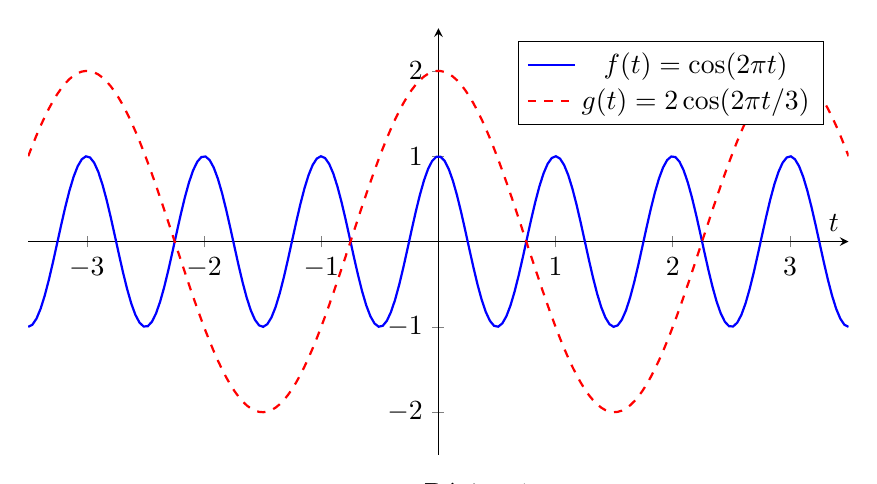
\begin{tikzpicture}
        \begin{axis}[
          axis lines=middle,
          xlabel={$t$},
          ylabel={},
          xmin=-3.5, xmax=3.5,
          ymin=-2.5, ymax=2.5,
          xtick={-3,-2,-1,0,1,2,3},
          ytick={-2,-1,0,1,2},
          width=12cm,
          height=7cm,
          samples=200,
          legend pos=north east,
        ]
        % f(t) = cos(2πt)
        \addplot[blue, thick, domain=-3.5:3.5] {cos(deg(2*pi*x))};
        \addlegendentry{$f(t) = \cos(2\pi t)$}
        
        % g(t) = 2cos(2πt/3)
        \addplot[red, thick, dashed, domain=-3.5:3.5] {2*cos(deg(2*pi*x/3))};
        \addlegendentry{$g(t) = 2\cos(2\pi t/3)$}
        \end{axis}
      \end{tikzpicture}
      \caption{Comparación de $f(t)$ y $g(t)$}
    \end{figure}
    
    Diría que $g(t)$ tiene la misma forma que $f(t)$ pero está estirada tanto en las direcciones vertical como horizontal. $f(t)$ tiene periodo 1 y amplitud 1, mientras que $g(t)$ tiene periodo 3 y amplitud 2.
    
    Usando la tasa de muestreo $2/3$ los puntos de muestra (según el teorema del muestreo) son $3k/2$. Los valores de $f(t)$ en los puntos de muestra son
    \begin{equation}
      f(3k/2) = \cos 2\pi \frac{3k}{2} = \cos 3k\pi = (-1)^k
    \end{equation}
    
    Los valores de $g(t)$ en los puntos de muestra son
    \begin{equation}
      g(3k/2) = 2\cos \frac{2\pi}{3} \frac{3k}{2} = 2\cos \pi k = 2(-1)^k
    \end{equation}
    
    $g(t)$ está ``siguiendo'' $f(t)$ en los puntos de muestra, pero las funciones no son iguales en esos puntos; $g(t)$ es el doble del tamaño. No llamaría a $g(t)$ un alias de $f(t)$ en el uso estándar del término.
  \end{solution}



\end{questions}
\end{document}